% Copyright (c)  2005-2010 EDF-EADS-PHIMECA.
% Permission is granted to copy, distribute and/or modify this document
% under the terms of the GNU Free Documentation License, Version 1.2
% or any later version published by the Free Software Foundation;
% with no Invariant Sections, no Front-Cover Texts, and no Back-Cover
% Texts.  A copy of the license is included in the section entitled "GNU
% Free Documentation License".
\renewcommand{\filename}{docUC_InputNoData_DistManipulation.tex}
\renewcommand{\filetitle}{UC : Manipulation of a distribution}

% \HeaderNNIILevel
% \HeaderIILevel
\HeaderIIILevel


\label{manipulation_distribution}


\index{Copula!Estimation from sample}
\index{Mixture}
\index{Graph!Specifying the file format}
\index{Graph!PDF-CDF curves}
\index{Graph!PDF-CDF isocurves}
\index{Graph Manipulation!Bounding box}
\index{Graph Manipulation!ViewImage}
\index{Graph Manipulation!Show}
\index{Quantile!Distribution evaluation}
\index{Sample Statistics!Sample Generation}



The objective of this Use Case is to describe the main functionalities that Open TURNS enables to manipulate a distribution of dimension $n \geq 1$.\\



Details on each object may be found in the User Manual  (\href{OpenTURNS_UserManual_TUI.pdf}{see User Manual - Probabilistic modeling}).\\


Let's note $\vect{X} = (X_1, \cdots, X_n)$ the random vector associated to that distribution, which PDF is note $p$. Open TURNS enables :
\begin{itemize}
\item to ask for the dimension, with the method {\itshape getDimension};
\item if $n >1$, to extract the extracted distribution of dimension $k<n$ corresponding to $k$ 1D marginals, with the method {\itshape getMarginal};
\item to get the copula, with the method {\itshape getCopula} : if the distribution is of type ComposedDistribution, the copula is the one specified at the creation of the ComposedDistribution. If the distribution is not that sort (for example, a KernelMixture, a Mixture, a RandomMixture), the copula is computed from the Sklar theorem;
\item to ask for some properties on the copula, with the method {\itshape hasIndependentCopula, hasEllipticalCopula}, only for the types Usual Distribution and ComposedDistribution (defined from the 1D marginals and a copula);
\item to evaluate the mean vector (potentially of dimension 1), the covariance matrix (potentially of dimension $1\times 1$), the standard deviation, skewness and kurtosis vectors (potentially of dimension 1), with the methods {\itshape getMean, getStandardDeviation, getCovariance, getKurtosis, getSkewness}, defined by the following expressions :
  $$
  \left\{
    \begin{array}{lcl}
      \displaystyle \vect{E}[\vect{X}] & = & \displaystyle (E[X_1], \cdots, E[X_n]) \\
      \displaystyle \mat{StdDev}[\vect{X}] & = & \displaystyle (\sqrt{E[(X_1-E[X_1])^2]}, \cdots, \sqrt{E[(X_n-E[X_n])^2]}) \\
      \displaystyle \mat{Cov}[\vect{X}] & = & \displaystyle (E\left[(X_i-E[X_i])(X_j-E[X_j])\right])_{i,j} \\
      \displaystyle \vect{skewness}[\vect{X}] & = & \displaystyle (E\left[\left(\frac{(X_1-E[X_1])}{\sqrt{Var[X_1]}}\right)^3\right], \cdots, E\left[\left(\frac{(X_n-E[X_n])}{\sqrt{Var[X_n]}}\right)^3\right]) \\
      \displaystyle \vect{kurtosis}[\vect{X}] & = & \displaystyle (E\left[\left(\frac{(X_1-E[X_1])}{\sqrt{Var[X_1]}}\right)^4\right], \cdots, E\left[\left(\frac{(X_n-E[X_n])}{\sqrt{Var[X_n]}}\right)^4\right])
    \end{array}
  \right.
  $$
\item to evaluate the roughness, with the method {\itshape getRoughness}, defined by :
  $$
  roughness(\vect{X}) = ||p||_{\mathcal{L}^2} = \sqrt{\int_\vect{x} p^2(\vect{x})d\vect{x}}
  $$

\item to get one realization or simultaneously $n$ realizations, with the method {\itshape getRealization, getNumericalSample},
\item to evaluate the Cumulative Distribution Function (CDF), the complementary CDF, the Probability Density Function (PDF) on a scalar (1D distribution only), on a point or on a numerical sample with the method {\itshape computeCDF, computePDF},
\item to evaluate the probability content of a given interval, with the method {\itshape computeProbability},
\item to evaluate a quantile or a complementary quantile, with the method {\itshape computeQuantile}. If the distribution if of dimension $n>1$, the $p-$ quantile is the hyper surface in $\mathbb{R}^n$ defined by  $\{\vect{x}\in \mathbb{R}^n, F(x_1, \dots, x_n) = p \}$ where $F$ is the CDF. Open TURNS makes the choice to return one particular point among these points : $(x_1^p, \dots, x_n^p)$ such that $\forall i, F_i(x_i^p) =  \tau$ where $F_i$ is the marginal of component $X_i$ and $F(x_1, \dots, x_n) = C(\tau, \dots, \tau)$ where $C$ is the distribution copula. Thus, Open TURNS resolves the equation $ C(\tau, \dots, \tau)=p$ then computes $F_i^{-1}(\tau) = x_i^p$.
\item to evaluate the derivative of the CDF or PDF with respect to the parameters of the distribution at a particular point, with the methods {\itshape computeCDFGradient, computePDFGradient},
\item to evaluate the characteristic function of the distribution, only for the following distributions : Chi2, Gamma, Laplace, Logistic, univariate Normal, Rayleigh, Triangular, univariate TruncatedNormal, Uniform, KernelMixture (which includes a KernelSmoothing without bound treatment), Mixture, RandomMixture;
\item to draw :
  \begin{itemize}
  \item for a 1D distribution : the PDF and CDF curves, with the methods {\itshape drawPDF, drawCDF},
  \item for a 2D distribution : the PDF and CDF iso-curves, with the methods {\itshape drawPDF, drawCDF}, and the PDF and CDF curves of its 1D marginals, with the methods {\itshape drawMarginal1DPDF, drawMarginal1DCDF} ,
  \item for a $nD$ with $n\geq 3$ distribution : the PDF and CDF of each 1D marginal, with the methods {\itshape drawMarginal1DPDF, drawMarginal1DCDF} and the PDF and CDF iso-curves for a specified 2D marginal, with the methods {\itshape drawMarginal2DPDF, drawMarginal2DCDF}.
  \end{itemize}
\end{itemize}

Let's note that it is possible to visualize a graph whithin the TUI without creating the associated files, thanks to the command {\itshape Show}.\\

\noindent%
\requirements{
  \begin{description}
  \item[$\bullet$] one distribution : {\itshape dist}
  \item[type:] Distribution
  \end{description}
}
{
  \begin{description}
  \item[$\bullet$] none
  \end{description}
}

\textspace\\
Python script for this UseCase :

\begin{lstlisting}

  # Get the dimension
  dim = dist.getDimension()
  print "Dimension of the distribution = ", dim

  # Get the marginals
  # the i-th marginal
  # Care : the numerotation begins at 0
  marginal_i = dist.getMarginal(i)

  # the marginal of the sub-distribution defined by several components
  # Put the indices of the concerned components together
  # for example, the three first components  (if dimension >2)
  TriDmarginal_123 = dist.getMarginal( (0,1,2) )

  # Get the copula
  copula = dist.getCopula()

  # Ask some properties on the copula
  print "hasIndependentCopula", dist.hasIndependentCopula
  print "hasEllipticalCopula", dist.hasEllipticalCopula

  # Get the mean vector of the distribution
  meanVector = dist.getMean()

  # Get the covariance matrix of the distribution
  meanVector = dist.getCovariance()

  # Get the kurtosis vector of the distribution
  kurtosisVector = dist.getKurtosis()

  # Get the standard deviation vector of the distribution
  standardDeviationVector = dist.getStandardDeviation()

  # Get the skewness vector of the distribution
  skewnessVector = dist.getSkewness()

  # Get the roughness of the distribution
  roughness = dist.getRoughness()

  # Get one realization of the distribution
  oneRealisationVector = dist.getRealization()

  # Get several realizations of the distribution
  # For example, 100 ones
  OneHundred_realizations = dist.getNumericalSample(100)

  # Evaluate the CDF and PDF
  # CARE : if the dimension is 1
  # For example, at pointValue=2.3
  pointValue = 2.3
  CDF_value = dist.computeCDF(pointValue)
  complementaryCDF_value = dist.computeCDF(pointValue, True)
  PDF_value = dist.computePDF(pointValue)

  # For the evaluation on a NumericalSample
  numSample = NumericalSample(2,1)
  numSample[0][0] = pointValue
  numSample[1][0] = 3*pointValue
  CDF_numSample = dist.computeCDF(numSample)
  PDF_numSample = dist.computePDF(numSample)

  # CARE : if the dimension is >1
  # For example, with dimension 2, at pointVector=(2.3, 4.5)
  pointVector = NumericalPoint( (2.3, 4.5) )
  CDF_vector = dist.computeCDF(pointVector)
  PDF_vector = dist.computePDF(pointVector)

  # Evaluate the probability content of an interval
  interval = Interval(-2.0, 3.0)
  probability = dist.computeProbability(interval)

  # Evaluate the quantile of order p
  # For example, the quantile 90%
  quantile_Vector_90 = dist.computeQuantile(0.90)
  complementaryQuantile_Vector_90 = dist.computeQuantile(0.90, True)

  # Evaluate the characteristic function of the distribution at pointVector
  complexResult = dist.computeCharacteristicFunction(pointVector)

  # Evaluate the derivatives of the PDF/CDF with respect to the parameters at a particular point
  # For example, with dimension 2, at pointVector=(2.3, 4.5)
  derivatives_PDF_Vector = dist.computePDFGradient(pointVector)
  derivatives_CDF_Vector = dist.computeCDFGradient(pointVector)


  # GRAPH 1 : Draw the PDF (CDF)  for a distribution of dimension 1

  # No specification of support
  PDF_1D_graph = dist.drawPDF()

  # Or Specify the support a and b (two scalars)
  # For example, a=-10.0 and b=10.0
  a=-10.0
  b=10.0
  PDF_1D_graph = dist.drawPDF(a,b)

  # Or impose a bounding box : x-range and y-range
  # boundingBox = [xmin, xmax, ymin, ymax]
  myBoundingBox = NumericalPoint( (xmin, xmax, ymin, ymax) )
  PDF_1D_graph.setBoundingBox(myBoundingBox)

  # In order to see the graph without creating the associated files
  Show(PDF_1D_graph)

  # Create the files corresponding to the graph
  # the files .EPS, .PNG and .FIG are created in the current python session
  PDF_1D_graph.draw("PDF_graph")

  # Or only the .EPS file
  # 640 and 480 are the pixels number in both axes
  PDF_1D_graph.draw("PDF_graph", 640, 480, GraphImplementation.EPS)

  # Visualize the PNG file within the TUI
  ViewImage(PDF_1D_graph.getBitmap())


  # GRAPH 2 :Draw the PDF (CDF) iso-curves for a distribution of dimension 2

  # No specification of support
  PDF_graph = dist.drawPDF()

  # Or Specify the support pointMin and pointMax
  # the graph will be drawn in the box with low-left corner : pointMin
  # and up-right corner : pointMax
  # For example, pointMin=(-3.0, -2.0) and pointMax=(4.0, 5.0)
  pointMin = NumericalPoint( (-3.0, -2.0) )
  pointMax = NumericalPoint( (4.0, 5.0) )

  # Specify the point number in each direction (curve look)
  pointNumber = NumericalPoint((201, 201))

  PDF_graph = dist.drawPDF(pointMin, pointMax, pointNumber)

  # Or impose a bounding box : x-range and y-range
  # boundingBox = [xmin, xmax, ymin, ymax]
  myBoundingBox = NumericalPoint( (xmin, xmax, ymin, ymax) )
  PDF_graph.setBoundingBox(myBoundingBox)


  # Change the default levels where the controus are drawn
  # Define the levels for example
  nlev = 31
  levels = NumericalPoint(nlev)
  for i in range(nlev):
  levels[i] = 0.25 * nlev / (1.0 + i)
  # Change them in the contour drawable
  PDF_graph_contour = PDF_graph.getDrawable(0)
  PDF_graph_contour.setLevels(levels)
  # If you don't need the labels on the iso curves
  PDF_graph_contour.setDrawLabels(False)

  PDF_graph.setDrawable(PDF_graph_contour,0)


  # In order to see the graph without creating the associated files
  Show(PDF_graph)

  # Create the files corresponding to the graph
  # the files .EPS, .PNG and .FIG are created in the current python session
  PDF_graph.draw("PDF_graph")

  # Or only the .EPS file
  # 640 and 480 are the pixels number in both axes
  PDF_graph.draw("PDF_isocurves_graph", 640, 480, GraphImplementation.EPS)

  # Visualize the PNG file in the TUI
  ViewImage(PDF_graph.getBitmap())


  # GRAPH 3 : Draw the PDF (CDF) of the 1D marginals for a distribution of dimension >=2

  # For example, marginal i
  # Care : the numerotation begins at 0

  # Specify the support a and b (two scalars) and the number of points of the curve
  # For example, a=-10.0 and b=10.0
  a = -10.0
  b = 10.0
  pointnumber = 101
  PDF_graph = dist.drawMarginal1DPDF(i, a, b, pointnumber)

  # Or impose a bounding box : x-range and y-range
  # boundingBox = [xmin, xmax, ymin, ymax]
  myBoundingBox = NumericalPoint( (xmin, xmax, ymin, ymax) )
  PDF_graph.setBoundingBox(myBoundingBox)

  # In order to see the graph without creating the associated files
  Show(PDF_graph)

  # Create the files corresponding to the graph
  # the files .EPS, .PNG and .FIG are created in the current python session
  PDF_graph.draw("PDF_graph")

  # Or only the .EPS file
  # 640 and 480 are the pixels number in both axes
  PDF_graph.draw("PDF_1DMarginals_graph", 640, 480, GraphImplementation.EPS)

  # Visualize the PNG file in the TUI
  ViewImage(PDF_graph.getBitmap())


  # GRAPH 4 : Draw the PDF (CDF) iso-curves for a distribution of dimension n>2

  # For example, the marginals i and j
  # Care : the numerotation begins at 0

  # Specify the support pointMin and  pointMax, and the number of points of the curve (all vectors)
  # For example, pointMin=(-3.0, -2.0) and pointMax=(4.0, 5.0)
  pointMin = NumericalPoint( (-3.0, -2.0) )
  pointMax = NumericalPoint( (4.0, 5.0) )
  pointNumber = NumericalPoint( (101, 101) )
  PDF_graph = dist.drawMarginal2DPDF(i, j, pointMin, pointMax, pointNumber)

  # Or impose a bounding box : x-range and y-range
  # boundingBox = [xmin, xmax, ymin, ymax]
  myBoundingBox = NumericalPoint( (xmin, xmax, ymin, ymax) )
  PDF_graph.setBoundingBox(myBoundingBox)

  # Change the default levels where the controus are drawn
  # Define the levels : for example
  nlev = 31
  levels = NumericalPoint(nlev)
  for i in range(nlev):
  levels[i] = 0.25 * nlev / (1.0 + i)
  # Change them in the contour drawable
  PDF_graph_contour = PDF_graph.getDrawable(0)
  PDF_graph_contour.setLevels(levels)
  # If you don't need the labels on the iso curves
  PDF_graph_contour.setDrawLabels(False)

  PDF_graph.setDrawable(PDF_graph_contour,0)


  # In order to see the graph without creating the associated files
  Show(PDF_graph)

  # Create the files corresponding to the graph
  # the files .EPS, .PNG and .FIG are created in the current python session
  PDF_graph.draw("PDF_2DMarginal_ij_graph")

  # Or only the .EPS file
  # 640 and 480 are the pixels number in both axes
  PDF_graph.draw("PDF_2DMarginal_ij_graph", 640, 480, GraphImplementation.EPS)

  # Visualize the PNG file in the TUI
  ViewImage(PDF_graph.getBitmap())
\end{lstlisting}
\textspace\\


We draw respectively  in Figures \ref{tulipe} and \ref{contour2D_example2} the iso-curves of the PDF of the two following  distributions :
\begin{itemize}
\item Distribution 1 : Mixture of Normal distributions of dimension 2
\item Distribution 2 : Composed Distribution, with a Gumbel copula and each marginal some mixture of normals of dimension 1.
\end{itemize}



\begin{figure}[H]
  \begin{center}
    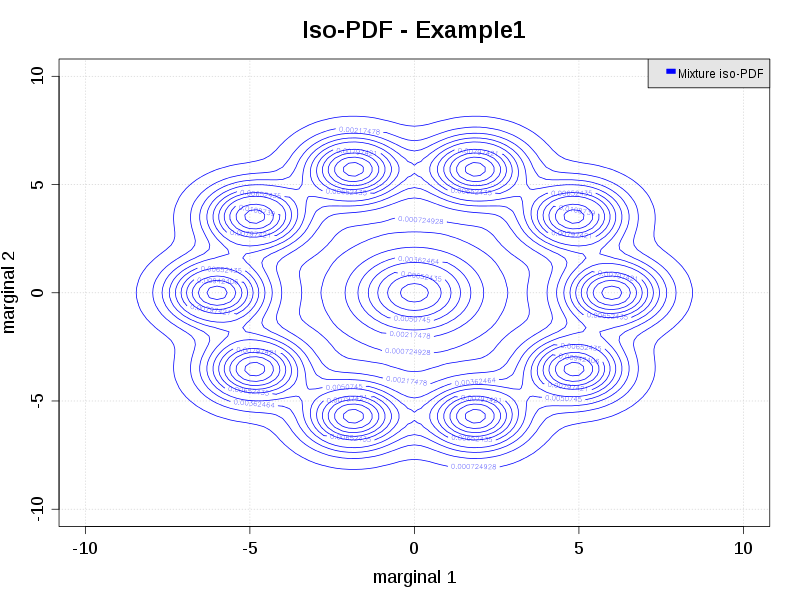
\includegraphics[width=10cm]{contour2D_tulipe.png}
  \end{center}
  \caption{Iso-curves of the PDF of Distribution 1 : Mixture of Normal distributions of dimension 2.}
  \label{tulipe}
\end{figure}

\begin{figure}[H]
  \begin{center}
    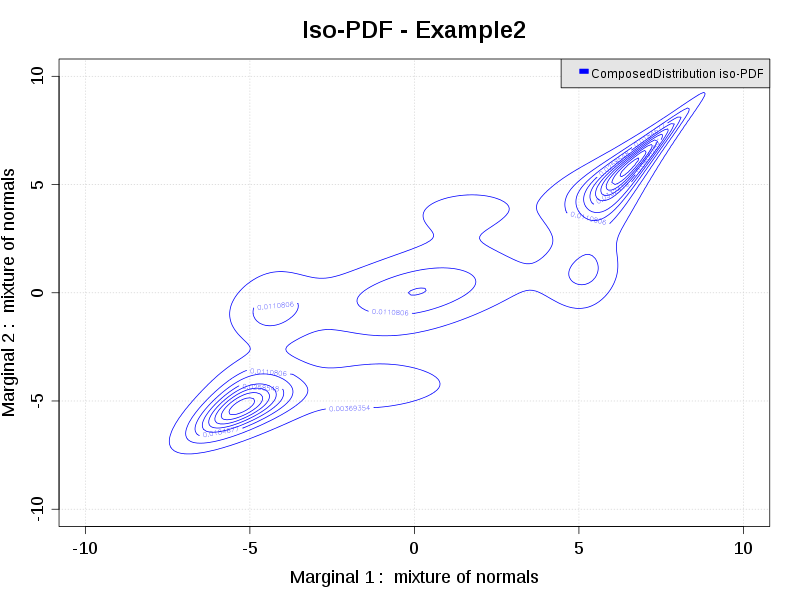
\includegraphics[width=10cm]{contour2D_2.png}
  \end{center}
  \caption{Iso-curves of the PDF of Distribution 2 : Composed Distribution, with a Gumbel copula and each marginal some mixture of normals of dimension 1.}
  \label{contour2D_example2}
\end{figure}


